\documentclass[relatorio.tex]{subfiles}
\begin{document}

\textit{Middleware}, como o nome indica, agrega toda a dinâmica que acontece entre o Servidor e o Cliente.
Utilizamos no sentido de mover ou transportar informações e dados entre programas de diferentes 
protocolos de comunicação e dependências do sistema operacional.

Assim, podemos definir como a comunicação entre o Servidor e o Cliente vai ocorrer.

\subsubsection{Gestão da Conexão}

A gestão desta conexão para suporte de diferentes padrões de interação por processos \textit{multithreaded}
é do âmbito da \textit{Tagged Connection} utilizada muito efetivamente durante as aulas.

\begin{minted}{java}
public class TaggedConnection implements AutoCloseable {

    private Socket s;
	protected DataInputStream in;
	protected DataOutputStream out;
	protected Lock sendLock = new ReentrantLock();
	protected Lock rcvLock = new ReentrantLock();
}
\end{minted}

Encontra-se definido o \textit{socket} a usar, usando \textbf{TCP}, \textit{streams} para permitir a
serialização e deserialização das mensagens entre os programas, e \textit{Locks}, para permitir vários 
pedidos e respostas serem efetuados concorrentemente, com o uso de \textit{Threads}.

Foi necessária a distinção entre a conexão por parte do Cliente e do Servidor, sendo criadas a:
\begin{itemize}
    \item \textit{Server Connection}
    \item \textit{Client Connection}
\end{itemize}

A razão para esta divisão foi devido ao método usado para o controlar as funcionalidades 
disponíveis aos utilizadores \textbf{administrativos} e \textbf{comuns}, auxiliando na autenticação
destes no sistema.
Cada cliente após se registar, obtém um \textit{Token} próprio e único a sí, \textit{encoded}.
Usando a biblioteca \textbf{JWT}, foi possível facilmente manusear este processo, e em cada \text{query}
efetuada pelo cliente, é inserida à cabeça o \textit{token} respetivo, para parametrizar
os utilizadores que estão a utilizar o sistema, e impedir que ocorram erros ao nível de 
funcionalidade administrativas erradamente disponíveis a utilizadores comuns.

Neste sentido, o \textit{Client Connection}:
\begin{minted}{java}
public class ClientConnection extends TaggedConnection {
  private String token;
}
\end{minted}

\subsubsection{Serialização}
Com a conexão entre o Servidor e o Cliente estabelecida, é de maior importância definir o tipo 
de mensagens a serem trocadas entre ambos, como um \textbf{protocolo}.

Antes do estado atual do sistema, encontrava-se definido que todas as mensagens a serem transmitidas
eram do tipo \textit{String}, sendo que facilitava a construção do programa, dado à sua simplicidade
de manuseamento.

Contudo, eram claras as limitações causadas por esta construção. Neste sentido, foi estabelecido uma 
dinâmica usando \textbf{DTOs}, ou \textit{Data-Transfer Objects}, trazendo um alto nível de flexibilidade
ao sistema.

\rightarrow \textbf{DTO}

Para o transporte de dados entre diferentes componentes, instâncias ou processos 
de um sistema distribuído ou diferentes sistemas via serialização, usa-se, caso da linguagem \textit{Java},
o conceito de um \textit{Data-Transfer Object}.

Neste caso, para serializar e deserializar as \textit{Queries} e \textit{Responses} do cliente e servidor, 
respetivamente, foi criado para cada uma o seu próprio DTO. 

Com o tipo primitivo \textbf{DTO},

\begin{minted}{java}
public abstract class DTO {    
    public abstract void serialize(DataOutputStream out) throws IOException;
}
\end{minted}

foram criados, adionalmente, nas suas \textit{packages} respetivas (\textit{QueryDTO} e \textit{ResponseDTO}),
ficheiros que controlam esta dinâmica de serialização/deserialização para cada um.
Permitindo que, no futuro, com a adição de novas funcionalidades, seja apenas necessária a adição dos seus 
\textit{DTOs} e não haja uma reestruturação do código.

\rightarrow \textbf{Frame}

Encontra-se na classe \textit{Frame}, o protótipo das mensagens enviadas.

\begin{minted}{java}
public class Frame {

    public final int tag;
    private final String className;
    private DTO dto;
}
\end{minted}

Com esta definição, explica-se o nome atribuído à conexão do Servidor/Cliente - \textit{Tagged Connection}, dado às mensagens serem etiquetadas,
neste caso, através da variável \textit{Tag}.
Possui o nome da classe (\textit{QueryDTO} e \textit{ResponseDTO}) que está a enviar e o respetivo DTO.


\subsubsection{Outros aspetos}

Encontram-se, também, dentro do \textit{Middleware}, várias exceções, para permitir que sejam lidadas ao nível do \textit{UI}.

Assim, como mencionado na estratégia utilizada (Ver \ref{strat_esc}), a conceção deste componente partiu de um diagrama, 
sendo este um \textbf{Diagrama de Classes}(Ver \ref{dig:classes_middle}).

\begin{figure}[H] \label{dig:classes_middle}
    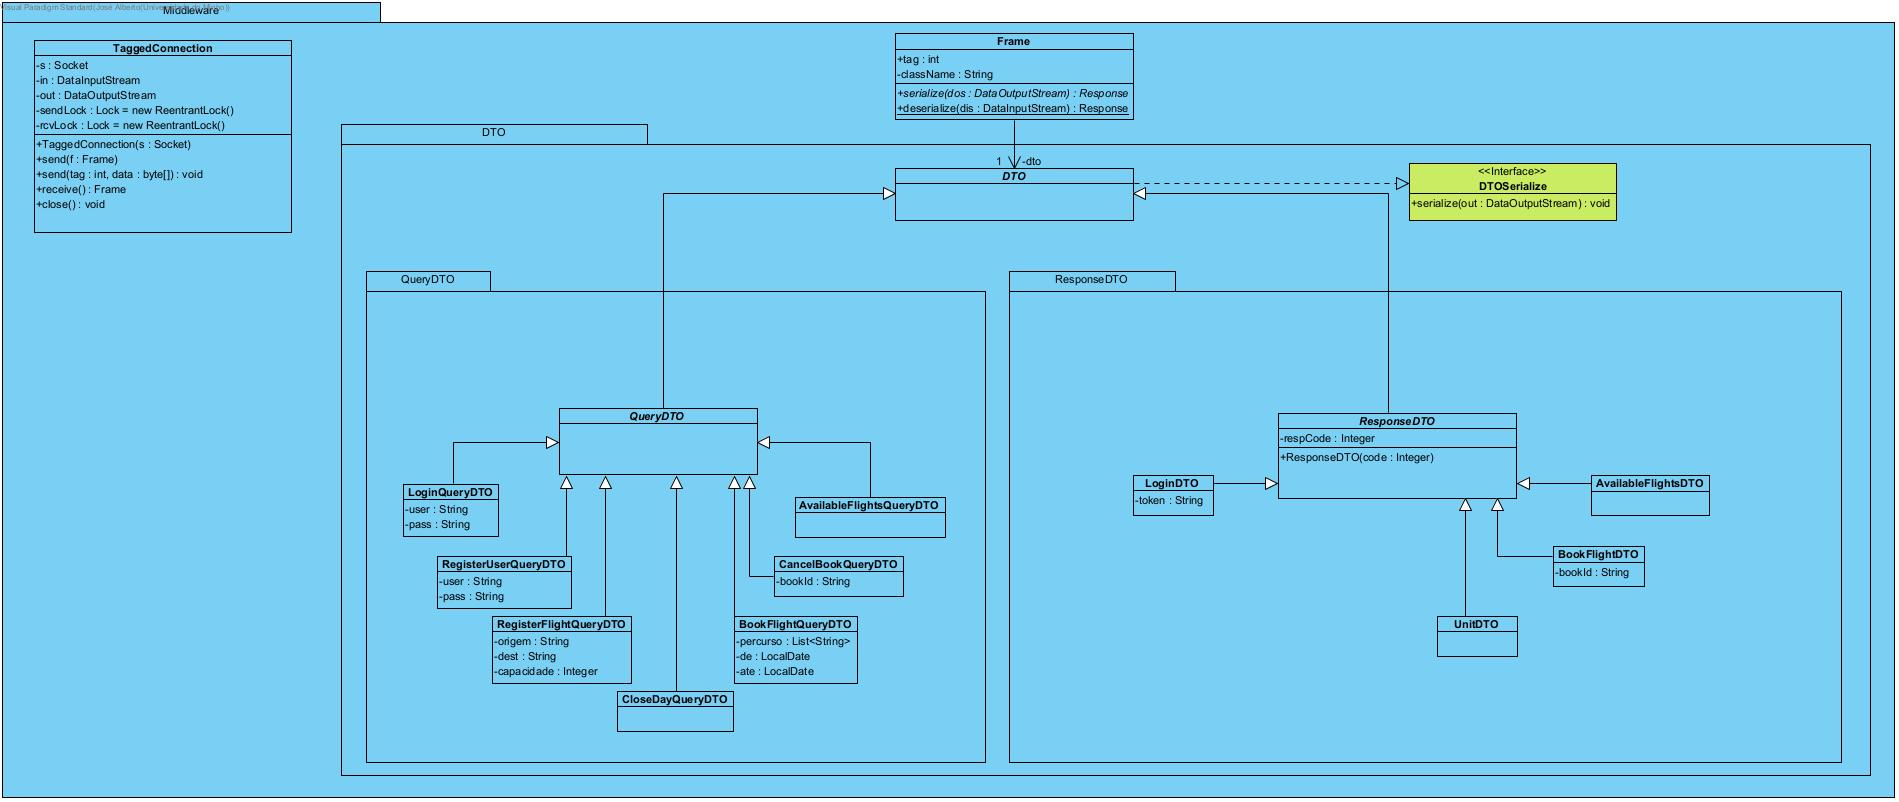
\includegraphics{diagrams/Middleware Class Diagram.jpg}
    \caption{Diagrama de classes para o \textit{Middleware}}
\end{figure}

Adicionalmente, foi construído um \textbf{Diagrama de Comunicações}, para definir a dinâmica (Ver \ref{dig:comms_middle}).

\begin{figure}{H} \label{dig:comms_middle}
    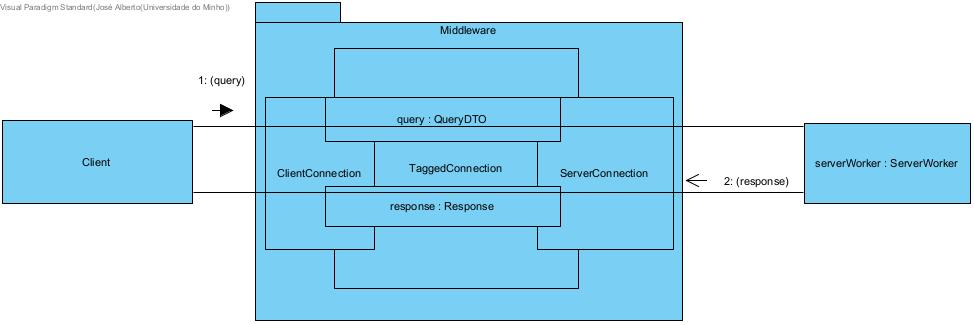
\includegraphics{diagrams/Middleware Communication Diagram.jpg}
    \caption{Diagrama de comuniações para o \textit{Middleware}}
\end{figure}

\end{document}